\documentclass[10pt]{article}
\usepackage{multicol}
\usepackage[letterpaper, total={6.6in, 9in}]{geometry}
\usepackage{indentfirst}
\usepackage{listings}
\usepackage{float}
\usepackage{graphicx}
\usepackage{inconsolata}
\usepackage{rosepine}
\PassOptionsToPackage{hyphens}{url}
\usepackage[obeyspaces, spaces]{url}
\makeatletter
\def\Url@space{\penalty\Url@sppen\hskip0.3em plus0.06em minus0.06em\relax}
\makeatother
\usepackage{hyperref}
\usepackage{cleveref}


\DeclareRobustCommand{\svdots}{% s for `scaling'
  \vbox{
    \baselineskip=0.33333\normalbaselineskip
    \lineskiplimit=0pt
    \hbox{.}\hbox{.}\hbox{.}
    \kern-0.2\baselineskip
  }
}

\title{User Manual for an Environmental Model Testing Framework}
\author{Sam Allen}
\date{\today}

\begin{document}

\maketitle
\begin{multicols}{2}

\section{Purpose}
Our goal is to determine how changing the values of model constants in the \verb|LakeTemperature| unit test module, a part of the Software Package for E3SM \cite{E3SM} Land (SPEL \cite{SPEL}), impacts that module's outputs. Additionally, we are testing to find faults in the module that result in physically impossible output values.

\section{Description}
Our environmental model testing framework is a Python program written to rapidly test many specific input combinations and quickly analyze the outputs. 

It includes support for both \textit{sampling} and \textit{analysis plugins}. Sampling plugins can be used to generate sets of model constant values to pass to the model, which is the executable created by SPEL to test the \verb|LakeTemperature| module in isolation. Analysis plugins take sets of output values and analyze them accordingly, generating human-readable console and file output, enabling researchers to easily interpret the results. 

\section{Terminology}
We introduce some terminology that will be used throughout the manual.
\begin{itemize}
    \item Model input: A variable that provides starting data for the model
    \item Model constant: A variable that controls how the  model behaves and manipulates data
    \item Model output: A variable that records data that the model has generated
    \item Sample: A set of values for the scalar model constants (which we can control during sample generation)
    \item Sample group: A grouping of samples arbitrarily ordered for convenience
    \item Sampling plugin: A custom way to create one or more sample groups on which to run \verb|LakeTemperature|
    \item Analysis plugin: A custom way to view and analyze model outputs that can either be run on each sample (\textit{per sample} analyzers) or run on all the samples in a sample group (\textit{sample group} analyzers)
\end{itemize}

\section{Installation}
Follow these steps to install the environmental testing framework:
\begin{enumerate}
    \item Get the dependencies: Python and Docker.
    \item Download and open the zip file of the application of the model testing framework to the \verb|LakeTemperature| module. Use the latest release or, if there are no releases, use the main branch. 
\begin{lstlisting}[style=dawn]
!> git clone https://github.com/SamAllen06/lake_temp_work.! !git!
\end{lstlisting}
    \item If you wish to extend the model testing framework, clone it using the following command:
\begin{lstlisting}[style=dawn]
!> git clone https://github.com/SamAllen06/model-testing-! !framework.git!
\end{lstlisting}
\end{enumerate}

\section{Configuration}
Running the testing framework involves picking the right sampling and analysis plugins based on the purpose of the application. First we will introduce all the sampling and analysis plugins currently supported by the tool. Then we will show how to configure the plugins before we run the testing framework. 
\subsection{Sampling Plugins}
Sampling plugins return one or more sample groups on which to run \verb|LakeTemperature|. They can be found in the repository at \path{testing/model_testing_framework/packages/sampling_plugins}. Our framework currently supports two sampling plugins. They are: 
\begin{itemize}
    \item NetCDF Cases: Creates sample groups from NetCDF \cite{NetCDF} files, a file format for self-describing datasets. We use this to run combinatorial test cases generated by the National Institute of Standards and Technology (NIST)'s ACTS \cite{ACTS} tool.
    \item Order Sampling: Creates sample groups using linear interpolation. We use this to to see the impact of changing a single model constant at a time on model outputs.
\end{itemize}

\subsection{Analysis Plugins}
Analysis plugins receive all model output data produced by either a single sample (per sample analyzers) or an entire sample group (sample group analyzers). They can be found in the repository at \path{testing/model_testing_framework/packages/analysis_plugins}. Our framework currently supports four analysis plugins. They are:
\begin{itemize}
    \item Per Sample Analyzers:
    \begin{itemize}
        \item Differences: Finds differences between values in the reference data and the current sample's data and then records the indices of the difference, the two differing values, and the difference between them
        \item Fault Finding: Uses functions defined by the plugin to make assertions about values in the sample data, similar to a unit testing framework but specialized to test model output values
    \end{itemize}
    
    \item Sample Group Analyzers:
    \begin{itemize}
        \item Change Detection: Identifies which model inputs and outputs differ from the reference across a whole sample group
        \item NetCDF4 Output: Stores output data from a sample group as a single NetCDF file
    \end{itemize}
\end{itemize}

\subsection{Whitelist}
The whitelist, as seen in \Cref{lst:whitelist_example}, determines which plugins are run. Only the plugins included in the whitelist will be run. This can be found in the repository at \path{testing/lake_temp/config/plugin_whitelist.json}.

\begin{lstlisting}[
    style=dawn,
    floatplacement=ht,
    caption=\texttt{plugin\_whitelist.json},
    label=lst:whitelist_example
]
{
    @@"sampling"@@: [
        !!"mtf_netcdf_cases"!!
    ],
    @@"analysis"@@: [
        !!"mtf_fault_finding"!!
    ]
}
\end{lstlisting}

\section{A Typical Run}
Follow these steps to run the model testing framework on the \verb|LakeTemperature| module:
\begin{enumerate}
    \item Open Docker.
    
    \item Run the \verb|LakeTemperature| testing script.
\begin{lstlisting}[style=dawn]
!> python testing/test_laketemperature.py
\end{lstlisting}

    \item Set the whitelist to the plugins you want.
    \begin{enumerate}
        \item Open the plugin whitelist in a text editor. Keep in mind that changes made from within a Docker container are not kept after the container is deleted. 
\begin{lstlisting}[style=dawn]
!> vim /app/config/plugin_whitelist.json
\end{lstlisting}
        \item Enter the names of the desired sampling and analysis plugins with ``mtf'' added to the beginning of each using snake case convention. For example, the differences plugin would be \verb|mtf_differences|.
        \item Save the file and quit the text editor. 
    \end{enumerate}

    \item If you want, alter how the whitelisted plugins will be run. 
    \begin{enumerate}
        \item Go to the directory of the desired plugin.
\begin{lstlisting}[style=dawn]
!> cd /app/plugin_inputs!
\end{lstlisting}
        \item Add or alter the files you want to be used and remove the files you don't want to be used for sampling and analysis. For example, \Cref{lst:combinatorial_example} shows a run where the NetCDF cases sampling plugin is altered by removing three files so that only \path{lake_temp_i2.nc} is used and the fault finding analysis plugin is altered by removing \path{finite_values_check.py} so its checks are not used.
    \end{enumerate}
    
    \item Run the model testing framework using the configurations stored in the \verb|config| directory.
\begin{lstlisting}[style=dawn]
!> mtf config!
\end{lstlisting}

    \item If you wish to run the loaded plugins, confirm using \verb|y| or \verb|Yes|. Capitalization doesn't matter. 
    
    \item Wait for the testing to finish. 
    
    \item Examine the output.
\begin{lstlisting}[style=dawn]
!> cd /app/testing/output/!
\end{lstlisting}

    \item Run \verb|exit| to exit the framework and delete the Docker container. 
\end{enumerate}

\section{Applications}
In this section, we'll demonstrate a few useful applications of the model testing framework to the \verb|LakeTemperature| module. 

\subsection{Combinatorial Testing}
To expose potential issues in the \verb|LakeTemperature| module that produce erroneous output, we used the framework to conduct combinatorial testing, demonstrated by \Cref{lst:combinatorial_example}. This method effectively reduces the number of test cases while ensuring pseudo-exhaustive testing to find problems in the code triggered by interactions of model constants. 

It accomplishes this by analyzing all interactions of only a small number of parameters, as NIST research found most software bugs are caused by interactions of only a few parameters \cite{ACTS}. 

We ran the combinatorial test cases generated by ACTS \cite{ACTS} using the NetCDF cases sampling plugin. Then we ran each sample's output through checks implemented via the fault finding analysis plugin. These check that the outputs fall within certain ranges, have certain signs, are finite, have certain relationships to other inputs and outputs, and follow physical laws and constraints. 

After analysis and before closing the Docker container, the output from the fault finding analysis plugin can be found in \path{/app/testing_output/analysis/sample/sample_group_name/`Mtf Fault Finding'}, where \texttt{sample\_group\_name} represents the name of a sample group which was run. For each test case, or sample, a directory is created which contains a file showing which checks passed, skipped, failed, or errored, a file showing which checks failed along with their error messages, a file for each check that errored, and a file containing the values of the model constants for the test case. 

\begin{lstlisting}[
    style=dawn,
    floatplacement=ht,
    caption=Combinatorial testing using the NetCDF cases sampling plugin and the fault finding analysis plugin,
    label=lst:combinatorial_example,
    escapechar=|
]
!> open -a Docker!
!> python testing/test_laketemperature.py!
[+] Building 8.9s (52/52) FINISHED
|\centerline{\texttt{\svdots}}|
!> vim config/plugin_whitelist.json!
!> rm plugin_inputs/netcdf_cases/lake_temp_i{3,4,5}.nc!
!> rm plugin_inputs/fault_checks/finite_values_check.py!
!> mtf config!
@Successfully loaded binary.@

Loading sampling plugins:
  @[Mtf Netcdf Cases]: Loaded@

Loaded 1 sampling plugin successfully. 

Loading analysis plugins:
  @[Mtf Fault Finding]: Loaded@

Loaded 1 analysis plugin successfully. 

Sampling from plugins:
  @[Mtf Netcdf Cases]:@
    lake_temp_i2: 231 samples
    Total: 1 group, 231 samples

  Grand Total: 1 group, 231 samples

Time estimated: 0:0:2:27
Would you like to continue? (Yes/No or y/n)
!> y!

Group 1 / 1: lake_temp_i2

Sample 1 / 231:
  betavis: 0.0
  cnfac: 0.0
  lake_no_ed: 1.0
  lakepuddling: 1.0
  use_1ch4: 1.0
  nlevlak: 2.4
  nlevgrnd: 2.5
  nevsno: 1.0
  nlevsoi: 1.5
  dtime_mod: 3520.0
  colia: 4181.0
  denh2o: 984.0
  tkwat: 0.1
  thk_bedrock: 2.2
  vkc: 0.1
  grav: 6.0
  hus: 333550.0
  denice: 915.5
  tkair: 0.012
  tkice: 1.2
  cpice: 2216.2
  iulog: 95.5
  pudz: 8.6
  miyfact: 0.27
  depthcrit: 17.0

@Binary ran successfully.@

Sample Analysis:
  @[Mtf Fault Finding]:@
    Results (45 checks run):
      @[PASSED]: 40 checks@
      ^[SKIPPED]: 5 checks^
|\centerline{\texttt{\svdots}}|
Sample 231 / 231:
  betavis: 0.30000000000000004
  cnfac: 1.0
  lake_no_end: 0.0
  lakepuddling: 1.0
  use_lch4: 1.0
  nlevlak: 13.6
  nlevgrnd: 22.5
  nlevsno: 4.0
  nlevsoi: 13.5
  dtime_mod: 3680.0
  clipq: 4189.0
  denh2o: 1016. 0
  tkwat: 0.9
  thk_bedrock: 3.8
  vkc: 6.000000000000001
  grav: 8.0
  hfus: 334000.0
  denice: 920.0
  tkair: 0.03
  tkice: 3.0
  cpice: 2218.0
  iulog: 100.0
  pudz: 14.0
  mixfact: 0.9
  depthcrit: 35.0

@Binary ran successfully.@

Sample Analysis: 
  @[Mtf Fault Finding]:@
    Results (45 checks run):
      @[PASSED]: 32 checks@
      ^[SKIPPED]: 6 checks^
      *[FAILED]: 7 checks*

    *[FAILED]: check_combined_heat_content_finite}*
      *Infinite or NaN values found in col_es%hc_soisno}*
    *[FAILED]: check_energy_conservation_residual_finite}*
      *Infinite or NaN values found in col_ef%errsoi}*
    *[FAILED]: check_ice_thickness_finite}*
      *Infinite or NaN values found in lakestate_vars%* *lake_icethick_col}*
    *[FAILED]: check_soil_heat_content_finite}*
      *Infinite or NaN values found in col_es%hc_soi}*
    *[FAILED]: check_soil_snow_temperature_finite}*
      *Infinite or NaN values found in col_es%t_soisno}*
    *[FAILED]: check_icethick_col_is_sum}*
      *Ice thickness is not consistent with other variables}*
    *[FAILED]: check_no_tke_when_surface_frozen}*
      *Turbulant kinetic energy present on a frozen surface*

Testing completed.
!> ls /app/testing_output/analysis/sample/lake_temp_i2/'Mtf Fault Finding'!
1   110 122 134 146 158 17  181 193 204 216 228 31  43  55  67  79  90
10  111 123 135 147 159 170 182 194 205 217 229 32  44  56  68  8   91
100 112 124 136 148 16  171 183 195 206 218 23  33  45  57  69  80  92
101 113 125 137 149 160 172 184 196 207 219 230 34  46  58  7   81  93
102 114 126 138 15  161 173 185 197 208 22  231 35  47  59  70  82  94
103 115 127 139 150 162 174 186 198 209 220 24  36  48  6   71  83  95
104 116 128 14  151 163 175 187 199 21  221 25  37  49  60  72  84  96
105 117 129 140 152 164 176 188 2   210 222 26  38  5   61  73  85  97
106 118 13  141 153 165 177 189 20  211 223 27  39  50  62  74  86  98
107 119 130 142 154 166 178 19  200 212 224 28  4   51  63  75  87  99
108 12  131 143 155 167 179 190 201 213 225 29  40  52  64  76  88
109 120 132 144 156 168 18  191 202 214 226 3   41  53  65  77  89
11  121 133 145 157 169 180 192 203 215 227 30  42  54  66  78  9
!> exit!
exit
\end{lstlisting}

\subsection{Change Detection}
To discover which model constants affect which model outputs, we implemented the change detection analysis plugin, demonstrated by \Cref{lst:order_sampling_change_detection_example}. Using the order sampling plugin, the values of a single model constant are changed across its range of values while keeping all other model constants at their default values. Lastly, the analysis plugin records all of the model outputs that changed as a result. 

This analysis was built on a few key assumptions: 
\begin{enumerate}
    \item Not all the model constants have an effect on the model outputs. 
    \item Model constants do not influence what values other model constants can take. 
    \item Model constants' effects on model outputs aren't determined by other preconditions being met.
\end{enumerate}
However, by discussing with the domain scientists and examining \verb|LakeTemperature| source code, these assumptions turned out to not hold, meaning the results of testing don't include all of the model outputs that the model constants affect. 

Nevertheless, it was still useful as it led to the discovery that certain constants only have an effect on model outputs under certain conditions. Additionally, the results are still valid and useful when specifically referring to the default values used in the test cases. 

After analysis and before closing the Docker container, the output from the change detection analysis plugin can be found in \path{/app/testing_output/analysis/group/sample_group_name/`Mtf Change Detection'}, where \texttt{sample\_group\_name} represents the name of a sample group which was run. For each sample group a directory is created which contains a file showing the names of all the model constants and a file showing which outputs changed. 

\begin{lstlisting}[
    style=dawn,
    floatplacement=ht,
    caption=Change detection using the order sampling plugin and the change detection analysis plugin,
    label=lst:order_sampling_change_detection_example,
    escapechar=|
]
!> open -a Docker!
!> python testing/test_laketemperature.py!
[+] Building 8.9s (52/52) FINISHED
|\centerline{\texttt{\svdots}}|
!> vim config/plugin_whitelist.json!
!> mtf config!
@Successfully loaded binary.@

Loading sampling plugins:
  @[Mtf Order Sampling]: Loaded@

Loaded 1 sampling plugin successfully. 

Loading analysis plugins:
  @[Mtf Change Detection]: Loaded@

Loaded 1 analysis plugin successfully. 

Sampling from plugins:
  @[Mtf Order Sampling]:@
    betavis_min_to_max: 11 samples
    Total: 1 group, 11 samples

  Grand Total: 1 group, 11 samples

Time estimated: 0:0:0:7
Would you like to continue? (Yes/No or y/n)
!> y!

Group 1 / 1: betavis_min_to_max

Sample 1 / 11:
  betavis: 0.0

@Binary ran successfully.@

Sample 2 / 11:
  betavis: 0.1

@Binary ran successfully.@
|\centerline{\texttt{\svdots}}|
Sample 11 / 11:
  betavis: 1.0

@Binary ran successfully.@

Group Analysis: 
  @[Mtf Change Detection]:@
    Changes to 11 outputs observed resulting from changes to a subset of the 28 constants. 

    Constants:
      tkwat
      mixfact
      use_lch4
      hfus
      nlevlak
      crop
      pudz
      lakepuddling
      dtime_mod
      cpice
      lake_no_ed
      grav
      tkice
      cnfac
      betavis
      nlevsoi
      percrop
      vkc
      nlevgrnd
      iulog
      iscft
      tkair
      depthcrit
      denice
      cpliq
      nlevsno
      thk_bedrock
      denh2o
    
    Outputs:
      col_es__hc_soisno
      col_es__t_lake
      lakestate_vars__betaprime_col
      veg_ef__eflx_sh_grnd
      lakestate_vars__lakeresist_col
      col_es__t_soisno
      veg_ef__eflx_soil_grnd
      ch4_vars__grnd_ch4_cond_col
      veg_ef__eflx_gnet
      col_es__hc_soi
      veg_ef__eflx_sh_tot

Testing completed.
!> ls /app/testing_output/analysis/group/betavis_min_to_max/'Mtf! !Change Detection'!
constants.txt  outputs.txt
!> exit!
exit
\end{lstlisting}

\subsection{Difference Analysis}
This analysis is similar to change detection except that it is performed on every individual sample, does not rely on the same assumptions, and it not only finds which outputs changed but records how much they changed from reference data (where all the constants take their default values), demonstrated by \Cref{lst:order_sampling_differences_example}.

This analysis records the differences between a single sample and the reference file. Consequently, the results are only valid within the context of the sample, reference, and values for the model inputs for the run. 

After analysis and before closing the Docker container, the output from the differences analysis plugin can be found in \path{/app/testing_output/analysis/sample/sample_group_name/`Mtf Differences'}, where \texttt{sample\_group\_name} represents the name of a sample group which was run. For each sample a directory is created which contains a text file showing which model outputs remained unchanged and a NetCDF file for each changed model output that shows where and by how much it differs from the reference. 

\begin{lstlisting}[
    style=dawn,
    floatplacement=ht,
    caption=Difference analysis using the order sampling plugin and the differences analysis plugin,
    label=lst:order_sampling_differences_example,
    escapechar=|
]
!> open -a Docker!
!> python testing/test_laketemperature.py!
[+] Building 52.3s (52/52) FINISHED
|\centerline{\texttt{\svdots}}|
!> vim config/plugin_whitelist.json!
!> mtf config!
@Successfully loaded binary.@

Loading sampling plugins:
  @[Mtf Order Sampling]: Loaded@

Loaded 1 sampling plugin successfully. 

Loading analysis plugins:
  @[Mtf Differences]: Loaded@

Loaded 1 analysis plugin successfully. 

Sampling from plugins:
  @[Mtf Order Sampling]:@
    betavis_min_to_max: 11 samples
    Total: 1 group, 11 samples

  Grand Total: 1 group, 11 samples

Time estimated: 0:0:0:9
Would you like to continue? (Yes/No or y/n)
!> y!

Group 1 / 1: betavis_min_to_max

Sample 1 / 11:
  betavis: 0.0

@Binary ran successfully.@

Sample Analysis:
  @[Mtf Differences]:@
    **No differences from reference found.**

Sample 2 / 11:
  betavis: 0.1

@Binary ran successfully.@

Sample Analysis:
  @[Mtf Differences]:@
    !!lakestate_vars__betaprime_col!!
    324 differences from reference found.
    !!col_es__t_soisno!!
    450 differences from reference found.
    !!col_es__t_lake!!
    540 differences from reference found.
    !!col_es__hc_soi!!
    54 differences from reference found.
    !!col_es__hc_soisno!!
    54 differences from reference found.
    !!veg_ef__eflx_sh_grnd!!
    54 differences from reference found.
    !!veg_ef__eflx_sh_tot!!
    54 differences from reference found.
    !!veg_ef__eflx_soil_grnd!!
    54 differences from reference found.
    !!veg_ef__eflx_gnet!!
    54 differences from reference found.
|\centerline{\texttt{\svdots}}|
Sample 11 / 11:
  betavis: 1.0

@Binary ran successfully.@

Sample Analysis:
  @[Mtf Differences]:@
    !!ch4_vars__grnd_ch4_cond_col!!
    1 difference from reference found.
    !!lakestate_vars__betaprime_col!!
    324 differences from reference found.
    !!lakestate_vars__lakeresist_col!!
    1 difference from reference found.
    !!col_es__t_soisno!!
    480 differences from reference found.
    !!col_es__t_lake!!
    540 differences from reference found.
    !!1col_es__hc_soi!!
    54 differences from reference found.
    !!col_es__hc_soisno!!
    54 differences from reference found.
    !!veg_ef__eflx_sh_grnd!!
    54 differences from reference found.
    !!veg_ef__eflx_sh_tot!!
    54 differences from reference found.
    !!veg_ef__eflx_soil_grnd!!
    54 differences from reference found.
    !!veg_ef__eflx_gnet!!
    54 differences from reference found.

Testing completed.
!> ls /app/testing_output/analysis/sample/betavis_min_to_max/'Mtf! !Differences'!
1  10  11  2  3  4  5  6  7  8	9
!> exit!
exit
\end{lstlisting}

\subsection{Change Impact Analysis}
In order to visualize the impact of changing a single model constant at a time on the model outputs, we paired the order sampling plugin with the NetCDF4 output analysis plugin, as shown in \Cref{lst:change_impact_example}.

We then used matplotlib to manually graph a single column from the output data, with time as the x-axis, the values of the model constant interpolated over as the y-axis, and the values of a single model output as the z-axis. Eventually this process will be made into a tool to automate graphing NetCDF4 output data but for \Cref{fig:example_graph} it was done manually. 

After analysis and before closing the Docker container, the output from NetCDF4 output analysis plugin can be found in \path{testing_output/analysis/group/sample_group_name/`Mtf Netcdf4 Output.nc'}, where \texttt{sample\_group\_name} represents the name of a sample group which was run. For each sample group a NetCDF file is created which contains all of the values for the model constants and model outputs across all of the samples in the sample group. 

\begin{figure}[H]
    \centering
    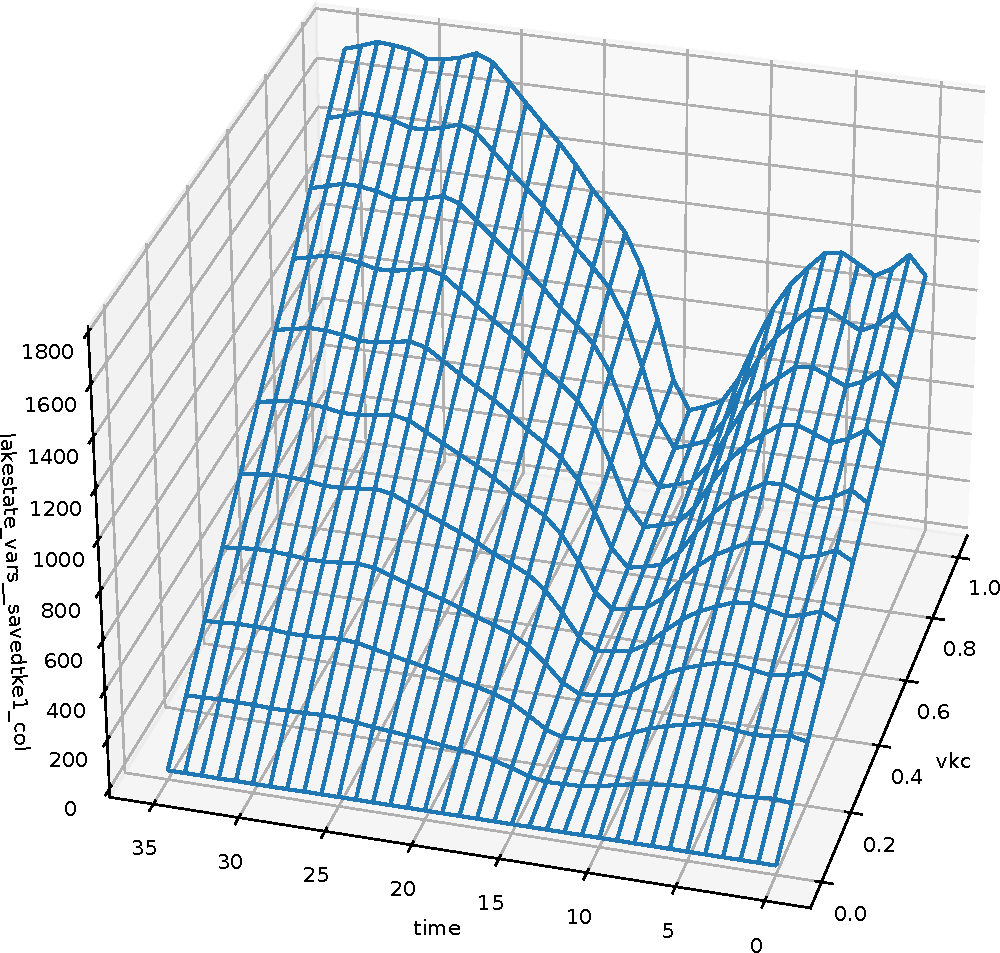
\includegraphics[width=0.8\linewidth]{change_impact.pdf}
    \caption{
        \texttt{saved\_tke1\_col} changing in response to a 
        change in \texttt{vkc}, a model constant
    }
    \label{fig:example_graph}
\end{figure}

\begin{lstlisting}[
    style=dawn,
    floatplacement=ht,
    caption=Change impact analysis using the order sampling plugin and the NetCDF4 output analysis plugin,
    label=lst:change_impact_example,
    escapechar=|
]
!> open -a Docker!
!> python testing/test_laketemperature.py!
[+] Building 44.2s (52/52) FINISHED
|\centerline{\texttt{\svdots}}|
!> vim config/plugin_whitelist.json!
!> mtf config!
@Successfully loaded binary.@

Loading sampling plugins:
  @[Mtf Order Sampling]: Loaded@

Loaded 1 sampling plugin successfully.

Loading analysis plugins:
  @[Mtf Netcdf4 Output]: Loaded@

Loaded 1 analysis plugin successfully.

Sampling from plugins:
  @[Mtf Order Sampling]:@
    vkc_min_to_max: 11 samples
    Total: 1 group, 11 samples

  Grand Total: 1 group, 11 samples

Time estimated: 0:0:0:7
Would you like to continue? (Yes/No or y/n)
!> y!

Group 1 / 1: vkc_min_to_max

Sample 1 / 11:
  vkc: 0.0

@Binary ran successfully. @

Sample 2 / 11:
  vkc: 0.1

@Binary ran successfully. @
|\centerline{\texttt{\svdots}}|
Sample 11 / 11:
  vkc: 1.0

@Binary ran successfully.@

Group Analysis:
  @[Mtf Netcdf4 Output]:@
    Success

Testing completed.
!> ls testing_output/analysis/group/vkc_min_to_max!
'Mtf Netcdf4 Output.nc'
!> exit!
exit
\end{lstlisting}

\section{Useful Tips and Troubleshooting}

\subsection{Creating CSV Test Cases}
We used ACTS \cite{ACTS} to generate our combinatorial test cases as CSV files. To avoid having to re-run the test case generation whenever we wanted to change the range of values used for each model constant, the ACTS cases were generated using indices that would later be mapped to actual values. Examples of CSV test case generation, the configuration file used for combinatorial test case generation, and the generated test cases in CSV format are given in \Cref{lst:creating_csv_test_cases_example}, \Cref{lst:conf_file_example}, and \Cref{lst:csv_test_cases_example}, respectively. 

This is demonstrated by the following steps:
\begin{enumerate}
    \item Download \verb|acts.jar| at \url{https://csrc.nist.gov/Projects/Automated-Combinatorial-Testing-for-Software/Downloadable-Tools}.

    \item Create the CSV test cases at the desired degree of interaction (DOI) using the configuration file.
\begin{lstlisting}[style=dawn]
!> java -jar -Ddoi=2|3|4|5 -Doutput=csv acts.jar! !test_resources/acts/all_constants/! !lake_temp_combinatorial.conf!
\end{lstlisting}

    \item Save the CSV test cases to \path{test_resources/acts/} in the \verb|lake_temp_work| repository.
\end{enumerate}

\begin{lstlisting}[
    style=dawn,
    floatplacement=ht,
    caption=An example of creating DOI 2 CSV test cases for all constants,
    label=lst:creating_csv_test_cases_example
]
!> java -jar -Ddoi=2 -Doutput=csv acts.jar test_resources/acts/! !all_constants/lake_temp_combinatorial.conf!
System Name: Lake Temperature SPEL Unit Test

Strength: 2
Mode: scratch
Algorithm: ipog
Constraing Handling: Ignored
Verify Coverage: off

Parameters      : 25
Constraints     : 0
Covered Tuples  : 28230 (2-way: 28230) 
Number of Tests : 231
Time (seconds)  : 0.041 

Output file: output.txt
!> mv output.txt test_resources/acts/all_constants/lake_temp_i2.csv!
\end{lstlisting}

\begin{lstlisting}[
    style=dawn,
    floatplacement=ht,
    caption= \texttt{lake\_temp\_combinatorial.conf},
    label=lst:conf_file_example,
    escapechar=|
]
[System]
Name: Lake Temperature SPEL Unit Test

[Parameter]
betavis (int) : 0, 1, 2, 3, 4, 5, 6, 7, 8, 9, 10
cnfac (int) : 0, 1, 2, 3, 4, 5, 6, 7, 8, 9, 10
lake_no_ed (int) : 0, 1
|\centerline{\texttt{\svdots}}|
depthcrit (int) : 0, 1, 2, 3, 4, 5, 6, 7, 8, 9, 10
\end{lstlisting}

\begin{lstlisting}[
    style=dawn,
    floatplacement=ht,
    caption=An example of CSV combinatorial test cases using indices,
    label=lst:csv_test_cases_example,
    escapechar=|
]
betavis,cnfac,lake_no_ed,lakepuddling,use_lch4,nlevlak,nlevgrnd,nlevsno,nlevsoi,dtime_mod,cpliq,denh2o,tkwat,thk_bedrock,vkc,grav,hfus,denice,tkair,tkice,cpice,iulog,pudz,mixfact,depthcrit
0, 0, 1, 1, 1, 1, 1, 1, 1, 1, 1, 1, 1, 1, 1, 1, 1, 1, 1, 1, 1, 1, 1, 1, 1
0, 1, 0, 0, 0, 2, 2, 2, 2, 2, 2, 2, 2, 2, 2, 2, 2, 2, 2, 2, 2, 2, 2, 2, 2
|\centerline{\texttt{\svdots}}|
3, 8, 0, 0, 1, 8, 8, 5, 8, 8, 8, 8, 8, 8, 7, 8, 10, 10, 10, 10, 10, 10, 10, 10, 10
3, 10, 0, 1, 1, 9, 9, 4, 9, 9, 9, 9, 9, 9, 6, 3, 10, 10, 10, 10, 10, 10, 10, 10, 10
\end{lstlisting}

\subsection{Converting CSV Test Cases to NetCDF Test Cases}
We used ACTS to generate our combinatorial test cases but its only options for output type are numeric, NIST, CSV, and Excel. To run \verb|Laketemperature| on our test cases using the NetCDF cases sampling plugin, we needed them to be in the form of a NetCDF file. The \verb|csv2nc| utility was used to convert CSV files to NetCDF files. This utility creates the NetCDF files using the values at the indices in the partition file that match the indices in the CSV test cases. Examples of the NetCDF case generation, the partition file used, the CSV cases, and the NetCDF cases are given in \Cref{lst:converting_csv_to_netcdf_example}, \Cref{lst:csv_test_cases_example}, \Cref{lst:partition_file_example}, and \Cref{lst:netcdf_test_cases_example}, respectively. 

The following steps demonstrate how to create the NetCDF combinatorial test cases:
\begin{enumerate}
    \item Create the CSV test cases if they have not already been made.
    \item Install the \verb|csv2nc| executable.
\begin{lstlisting}[style=dawn]
!> pip install testing/utils/acts_csv_to_ncdf_cases!
\end{lstlisting}
    \item Convert the CSV test cases to NetCDF files using the \verb|csv2nc| utility.
\end{enumerate}

\begin{lstlisting}[
    style=dawn,
    floatplacement=ht,
    caption=An example of converting DOI 2 CSV test cases to NetCDF test cases for all constants,
    label=lst:converting_csv_to_netcdf_example,
    escapechar=|
]
!> csv2nc test_resources/acts/all_constants/lake_temp_i2.csv! !test_resources/acts/all_constants/lake_temp_partition.nc! !test_resources/acts/all_constants/lake_temp_i2.nc!
\end{lstlisting}

\begin{lstlisting}[
    style=dawn,
    floatplacement=ht,
    caption=\texttt{lake\_temp\_partition.nc},
    label=lst:partition_file_example,
    escapechar=|
]
dimensions:
  betavis_test_value = 11 ;
  cnfac_test_value = 11 ;
  lake_no_ed_test_value = 2 ;
|\centerline{\texttt{\svdots}}|
  depthcrit_test_value = 11 ;
variables:
  double betavis(betavis_test_value) ;
  double cnfac(cnfac_test_value) ;
  double lake_no_ed(lake_no_ed_test_value) ;
|\centerline{\texttt{\svdots}}|
  double depthcrit(depthcrit_test_value) ;
data:
  betavis = 0, 0.1, 0.2, 0.3, 0.4, 0.5, 0.6, 0.7, 0.8, 0.9, 1 ;
  cnfac = 0, 0.1, 0.2, 0.3, 0.4, 0.5, 0.6, 0.7, 0.8, 0.9, 1 ;
  lake_no_ed = 0, 1 ;
|\centerline{\texttt{\svdots}}|
  depthcrit = 15, 17, 19, 21, 23, 25, 27, 29, 31, 33, 35 ;
\end{lstlisting}

\begin{lstlisting}[
    style=dawn,
    floatplacement=ht,
    caption=An example of NetCDF combinatorial test cases,
    label=lst:netcdf_test_cases_example,
    escapechar=|
]
dimensions:
  cases = UNLIMITED ; // (231 currently)
variables:
  double betavis(cases) ;
  double cnfac(cases) ;
  double lake_no_ed(cases) ;
|\centerline{\texttt{\svdots}}|
  double depthcrit(cases) ;
data:
  betavis = 0, 0, 0, 0, 0, ..., 0.8, 0.4, 0.4, 0.3, 0.3 ;
  cnfac = 0, 0.1, 0.2, 0.3, 0.4, ..., 0.5, 0.6, 0.7, 0.8, 1 ;
  lake_no_ed = 1, 0, 1, 0, 1, ..., 1, 0, 1, 0, 0 ;
|\centerline{\texttt{\svdots}}|
  depthcrit = 17, 19, 21, 23, 25, ..., 35, 35, 35, 35, 35 ;
\end{lstlisting}

\subsection{Summarizing Fault Finding Analysis Plugin Output}
Since the fault finding analysis plugin creates an output directory for every sample run (which can range from 231 to 1,009,602 when using the combinatorial test cases), an additional utility can be manually run to summarize all of the output data into a single console text output.

The output will include the number of sample runs that exited with an error, how many samples passed, skipped, failed, and errored for every check, and a list of which samples passed, skipped, failed, and errored for every single fault check. An example is given by \Cref{lst:summarize_utility_example}. 

The following steps are used to summarize fault finding analysis plugin output:
\begin{enumerate}
    \item Run \path{testing/test_laketemperature.py} on the NetCDF cases sampling plugin and the fault finding analysis plugin. 
    \item From a separate terminal, copy the desired output files at \path{"/app/testing_output/analysis/sample"} from the Docker container to your local device.
    \item Run the summarize utility in the repository at \path{testing/utils/fault_check_summarize/src/fcsum/main.py} on the output directory, including the total number of samples run. 
\end{enumerate}

\end{multicols}
\begin{lstlisting}[
    style=dawn,
    % float=tp,
    caption=An example of running the summarize utility on DOI 2 all constants output data,
    label=lst:summarize_utility_example,
    escapechar=?,
    columns=fixed
]
!> docker cp container_id:/app/testing_output/analysis/sample/lake_temp_i2/"Mtf Fault Finding" my_local_directory!
!> python testing/utils/fault_check_summarize/src/fcsum/main.py my_local_directory 231!
0 out of 231 runs exited with an error.
| Check                                                       | Passed | Skipped | Failed | Errored |
| check_combined_heat_content_finite                          | 115    | 0       | 116    | 0       |
?\centerline{\texttt{\svdots}}?
| check_temp_around_freezing_where_lake_is_almost_frozen      | 0      | 231     | 0      | 0       |
| check_total_sensible_heat_flux_finite                       | 231    | 0       | 0      | 0       |
| check_water_snow_equivalent_not_negative                    | 231    | 0       | 0      | 0       |

Samples per result:
| check_combined_heat_content_finite FAILED:                                                        |
|     7, 8, 9, 10, 11, 16, 17, 18, 19, 20, 25, 26, 27, 28, 29, 30, 34, 35, 36, 37, 38, 39, 40, 45,  |
|     46, 48, 49, 50, 54, 55, 58, 59, 60, 63, 64, 65, 66, 68, 69, 70, 72, 73, 74, 75, 78, 79, 80,   |
|     81, 82, 83, 84, 89, 90, 91, 92, 93, 99, 100, 101, 102, 109, 110, 111, 119, 120, 121, 128,     |
|     129, 130, 131, 132, 138, 139, 140, 141, 142, 148, 149, 150, 151, 152, 158, 159, 160, 161,     |
|     162, 168, 169, 170, 171, 172, 178, 179, 180, 181, 182, 188, 189, 190, 191, 192, 199, 200,     |
|     201, 202, 209, 210, 211, 212, 219, 220, 221, 222, 229, 230, 231                               |
?\centerline{\texttt{\svdots}}?
| check_water_snow_equivalent_not_negative PASSED:                                                  |
|     1, 2, 3, 4, 5, 6, 7, 8, 9, 10, 11, 12, 13, 14, 15, 16, 17, 18, 19, 20, 21, 22, 23, 24, 25,    |
|     26, 27, 28, 29, 30, 31, 32, 33, 34, 35, 36, 37, 38, 39, 40, 41, 42, 43, 44, 45, 46, 47, 48,   |
|     49, 50, 51, 52, 53, 54, 55, 56, 57, 58, 59, 60, 61, 62, 63, 64, 65, 66, 67, 68, 69, 70, 71,   |
|     72, 73, 74, 75, 76, 77, 78, 79, 80, 81, 82, 83, 84, 85, 86, 87, 88, 89, 90, 91, 92, 93, 94,   |
|     95, 96, 97, 98, 99, 100, 101, 102, 103, 104, 105, 106, 107, 108, 109, 110, 111, 112, 113,     |
|     114, 115, 116, 117, 118, 119, 120, 121, 122, 123, 124, 125, 126, 127, 128, 129, 130, 131,     |
|     132, 133, 134, 135, 136, 137, 138, 139, 140, 141, 142, 143, 144, 145, 146, 147, 148, 149,     |
|     150, 151, 152, 153, 154, 155, 156, 157, 158, 159, 160, 161, 162, 163, 164, 165, 166, 167,     |
|     168, 169, 170, 171, 172, 173, 174, 175, 176, 177, 178, 179, 180, 181, 182, 183, 184, 185,     |
|     186, 187, 188, 189, 190, 191, 192, 193, 194, 195, 196, 197, 198, 199, 200, 201, 202, 203,     |
|     204, 205, 206, 207, 208, 209, 210, 211, 212, 213, 214, 215, 216, 217, 218, 219, 220, 221,     |
|     222, 223, 224, 225, 226, 227, 228, 229, 230, 231                                              |
\end{lstlisting}

\begin{multicols}{2}

\subsection{Documentation}
There are a few places where documentation can be found to help with understanding the application of the model testing framework to \verb|LakeTemperature| and extending the model testing framework to be used in new contexts. 

For the \verb|lake_temp_work| repository, all documentation (except for the \path{README.md} file) can be found in the \path{documentation} directory. This directory contains a wide range of documentation used by us in creating the application of the model testing framework to the \verb|LakeTemperature| module. For example, it has documentation regarding the implementation of the fault checks, the \verb|csv2nc| and \verb|fault_check_summarize| utilities, documents we've created for our collaborators at Oak Ridge National Laboratory, documents we've received from our collaborators, a conference paper we wrote, and more. It is useful for understanding the \verb|lake_temp_work| repository. 

For the \verb|model-testing-framework| repository, all documentation (except for the \path{README.md} file) can be found in the \path{docs} directory. This contains documentation about things such as existing analysis and sampling plugins, how to configure analysis and sampling plugins, the whitelist, console and file output, and more. This would be useful when creating plugins or extending the model testing framework to be used in a specific context, like we have with the \verb|LakeTemperature| module. 

\subsection{Changing the Number of Time Steps}
Line 46 in \path{testing/Dockerfile} in the repository is used to run \verb|LakeTemperature| for a custom number of time steps. It is currently set to 35, which makes the program run quicker and allows us to expose issues with our framework while debugging it. 

The number ``35'' can be changed to however many time steps you want to run \verb|LakeTemperature| for. Alternatively, you can comment out line 46 entirely to run \verb|LakeTemperature| for the default of 1,000 time steps, which will make the testing take longer but will also help expose more issues within the \verb|LakeTemperature| module. 

\subsection{Reading a NetCDF File's Contents}
Since the framework makes frequent use of NetCDF files, it is useful to be able to examine their contents. Start by installing NetCDF4 to your device. 
\begin{lstlisting}[style=dawn]
!> pip install netCDF4!
\end{lstlisting}

View the entire file using \verb|ncdump| \path{file_name.nc}, view header information only using \verb|ncdump -h| \path{file_name.nc}, and view specific variables only using \verb|ncdump -v variable_name| \path{file_name.nc}. To find all other commands, use \verb|ncdump -h|. 

\subsection{Copying Files from a Docker Container}
Since the framework makes frequent use of Docker containers, it is useful to be able to copy files from and to an existing Docker container. 

After running and before exiting \path{testing/test_laketemperature.py} and using a separate terminal, enter \verb|docker cp container_id:|\path{/app/SRC_PATH} \path{DEST_PATH} to copy a file from a Docker container and enter \verb|docker cp| \path{SRC_PATH} \verb|container_id:|\path{/app/DEST_PATH} to copy a file to a Docker container. 

\subsection{Debugging}
The Python debugger is a useful tool for finding issues in the model testing framework and its application to \verb|LakeTemperature|. Just add \verb|import pdb| to the desired file and insert \verb|pdb.set_trace()| where you would like the program to stop and enter the debugging interface. 

\subsection{Forgetting to Open Docker}
If the Docker app is not open, the \path{testing/test_laketemperature.py} script will not be able to run. To fix this, just make sure the Docker app is open before running \path{testing/test_laketemperature.py}. \Cref{lst:docker_error_example} shows a representation of this problem and its solution. 

\begin{lstlisting}[
    style=dawn,
    floatplacement=ht,
    caption=An example of a Docker API error,
    label=lst:docker_error_example
]
!> python testing/test_laketemperature.py!
failed to connect to the docker API
!> open -a Docker!
!> python testing/test_laketemperature.py!
[+] Building 8.9s (52/52) FINISHED
\end{lstlisting}

\bibliographystyle{bib/latex8}
\bibliography{bib/manual.bib}

\end{multicols}

\end{document}